\begin{enumerate}

%appL
\item $M \to_\beta M_2$ es $PZ \to_\beta P_1 Z$
\begin{figure}[h]
\centering
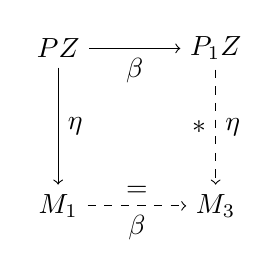
\begin{tikzpicture}
  \node (A) at (0, 2) {$PZ$};
  \node (B) at (2, 2) {$P_1 Z$};
  \node (C) at (0, 0) {$M_1$};
  \node (D) at (2, 0) {$M_3$};
  \draw[->] (A) -- node[below] {$\beta$}  (B);
  \draw[->] (A) -- node[right] {$\eta$} (C);
  \draw[->, dashed] (B)-- node[right] {$\eta$} node[left] {$*$} (D);
  \draw[->, dashed] (C)-- node[below]  {$\beta$} node[above] {$=$} (D);
\end{tikzpicture}
\end{figure}

Hipótesis de inducción:
\begin{figure}[h]
\centering
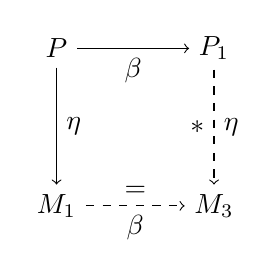
\begin{tikzpicture}
  \node (A) at (0, 2) {$P$};
  \node (B) at (2, 2) {$P_1$};
  \node (C) at (0, 0) {$M_1$};
  \node (D) at (2, 0) {$M_3$};
  \draw[->] (A) -- node[below] {$\beta$}  (B);
  \draw[->] (A) -- node[right] {$\eta$} (C);
  \draw[->, dashed] (B)-- node[right] {$\eta$} node[left] {$*$} (D);
  \draw[->, dashed] (C)-- node[below]  {$\beta$} node[above] {$=$} (D);
\end{tikzpicture}
\end{figure}
\newpage
%appR
\item $M \to_\beta M_2$ es $ZP \to ZP_1$
\begin{figure}[h]
\centering
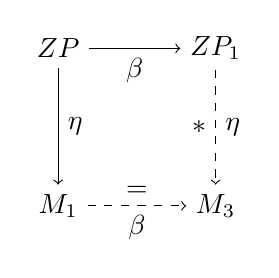
\begin{tikzpicture}
  \node (A) at (0, 2) {$ZP$};
  \node (B) at (2, 2) {$Z P_1$};
  \node (C) at (0, 0) {$M_1$};
  \node (D) at (2, 0) {$M_3$};
  \draw[->] (A) -- node[below] {$\beta$}  (B);
  \draw[->] (A) -- node[right] {$\eta$} (C);
  \draw[->, dashed] (B)-- node[right] {$\eta$} node[left] {$*$} (D);
  \draw[->, dashed] (C)-- node[below]  {$\beta$} node[above] {$=$} (D);
\end{tikzpicture}
\end{figure}

Hipótesis de inducción:
\begin{figure}[h]
\centering
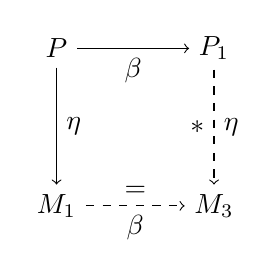
\begin{tikzpicture}
  \node (A) at (0, 2) {$P$};
  \node (B) at (2, 2) {$P_1$};
  \node (C) at (0, 0) {$M_1$};
  \node (D) at (2, 0) {$M_3$};
  \draw[->] (A) -- node[below] {$\beta$}  (B);
  \draw[->] (A) -- node[right] {$\eta$} (C);
  \draw[->, dashed] (B)-- node[right] {$\eta$} node[left] {$*$} (D);
  \draw[->, dashed] (C)-- node[below]  {$\beta$} node[above] {$=$} (D);
\end{tikzpicture}
\end{figure}

\end{enumerate}


